
In this appendix, we present the results of our analysis on the experimental single-cell data provided by \cite{yvert-et-al-2013}. We assume that the reader is aware of the basic definitions and equations provided in the main manuscript.

\cite{yvert-et-al-2013} used automated image analysis to describe yeast phenotypic diversity at a single-cell resolution (known as phenomics, \citealt{ohya-et-al-2015}). They monitored $n=125$ phenotypic characters on isogenic populations of $m=37$ different strains of yeast, living in natural or laboratory conditions. For each strain, they measured 5 replicates of approximately 200 cells each ($\sim$1000 cells per strain). They demonstrated that phenotypic noise significantly differs between strains, supporting ``\textit{the possibility that, if noise is adaptive, microevolution may tune it in the wild}'' \citep{yvert-et-al-2013}.

We used the raw datasets published by the authors to measure intra-strain (\textit{i.e.} isogenic) noise correlations between characters. The goal of our study is to test the existence of correlated phenotypic noise in natural strains of yeast. The datasets provided by \cite{yvert-et-al-2013} are structured as following: for each strain of yeast, a set of files is provided in a dedicated folder (a dataset per replicate). For each replicate, the list of single-cell measures is dispatched in three different files in \texttt{xls} format. Each cell is identified by a unique tag per image and the tag of the captured image. Each time a measure failed (on one character, or on the entire cell), the corresponding element (or line) in the table was filled with value $-1$.
Several characters are redundant (for example the volume and the size of the nucleus), and strongly correlated. Moreover, each trait value is provided with specific units (\textit{e.g.}, number of pixels, volume or angle units), such that some normalization is necessary.
The code associated to this analysis is freely available in Script \ref{part1:ScriptS2}. One can run again the whole analysis by following instructions provided in the README file. The raw dataset is freely provided by \cite{yvert-et-al-2013}.

The purpose of the analysis is to determine whether intra-strain variability presents correlations between characters \textit{once inter-strain correlations  between characters have been removed}. 

Let us first process inter-strain variability. The idea is to find a phenotypic space in which there is as little character-specific variability and correlation as possible. Here we have 37 isogenic strains, hence 37 genotypes. We define the ``phenotype'' of a strain/genotype as the vector of mean trait values, computed over all cells from this strain/genotype. We then define the ``centered phenotype" of a strain/genotype by removing the grand mean of each character. The singular value decomposition of the 37x125 matrix of centered strain phenotypes will give us a set of orthonormal linear combinations of characters. By construction, when the centered strain phenotypes are expressed according to these new characters, they lose all their pairwise correlations, implying that the variance-covariance matrix is diagonal for those new characters. Moreover, we normalize the variance of each new strain phenotype to one\footnote{Which is why our analysis is not exactly a PCA: We drop the singular values that are usually left in the PCA.}, such that the 37 new strain phenotypes are isotropically distributed.

This new base is the closest analogy we could think of to the phenotypic space in the classical version of Fisher's geometric model. Fisher's phenotypic space is orthogonal and normalized, and mutations on the genotype cause phenotypic traits to vary independently and with the same amplitude, according to an isotropic mutational distribution.

The second step is to project intra-strain single-cell data in Fisher's space, and to analyze the possible remaining correlations of intra-strain phenotypic variability in this space.

Figure \ref{part1:appendixS1:fig1} shows the detailed steps of our analysis, as described  below. First, we converted each \texttt{xls} file into \texttt{csv} format, and we merged the three files of each replicate to obtain a single dataset $\boldsymbol{M_{0,s,r}}$ ($s \in \{1,...,37\}$, $r \in \{1,...,5\}$) per replicate, and we removed useless information (such as cell identifiers, coordinates on the image, and so on) (Fig. \ref{part1:appendixS1:fig1}.1).
Then we merged the 5 replicates of each strain (Fig. \ref{part1:appendixS1:fig1}.2) to compute the matrix $\boldsymbol{M_0}$ of the mean phenotypic characters per strain (Fig. \ref{part1:appendixS1:fig1}.3).
Each column ${\boldsymbol{M_0}}_j$ of $\boldsymbol{M_0}$ was centered and normalized to obtain the matrix $\boldsymbol{M}$ (Fig. \ref{part1:appendixS1:fig1}.4):
\begin{equation}
{\boldsymbol{M}}_j = \dfrac{{\boldsymbol{M_0}}_j-\mathrm{mean}({\boldsymbol{M_0}}_j)}{\mathrm{stdev}({\boldsymbol{M_0}}_j)}.
\end{equation}
We also standardized each replicate to obtain $37\times5$ matrices $M_{s,r}, s \in \{1,...,37\}, r \in \{1,...,5\}$ (Fig. \ref{part1:appendixS1:fig1}.6). For each column ${\boldsymbol{M_{0,s,r}}}_j$ of $\boldsymbol{M_{0,s,r}}$:
\begin{equation}
{\boldsymbol{M_{s,r}}}_j = \dfrac{{\boldsymbol{M_{0,s,r}}}_j-\mathrm{mean}({\boldsymbol{M_{0,s,r}}}_j)}{\mathrm{stdev}({\boldsymbol{M_{0,s,r}}}_j)}.
\end{equation}
To find Fisher's space, we computed a SVD from $\boldsymbol{M}$ (see details below, and Fig. \ref{part1:appendixS1:fig1}.5).
For each standardized replicate dataset $\boldsymbol{M_{s,r}}$, many trait values are missing, and are replaced by $-1$ values, making impossible some mathematical operations. For this reason, a next step was to estimate the missing values: we used a simple conservative method, as described below (Fig. \ref{part1:appendixS1:fig1}.7). Finally, each replicate dataset was projected in Fisher's space (Fig. \ref{part1:appendixS1:fig1}.8). The inter-replicate variability was evaluated to ensure that experimental variability is low enough (Fig. \ref{part1:appendixS1:fig1}.9), and intra-strain phenotypic noise correlations were analyzed (Fig. \ref{part1:appendixS1:fig1}.10).

We describe below the steps requiring details.

%%%%%%%%%%%%%%%%%
%%%%%%%%%%%%%%%%%

\section*{Estimation of missing values}
To estimate missing values, we first computed the cell-to-cell Pearson correlation matrix $\boldsymbol{C}$ associated to each replicate, based on available data.
Knowing there are $m' \sim 200$ cells and $n=125$ phenotypic characters in each replicate, we defined a cell by a vector $\boldsymbol{X_i} \in \mathbb{R}^{125}$, with $i \in \{1,...,m'\}$.

Each missing value $x_{i,j}$ of $\boldsymbol{X_i}$ (with $j \in \{1,...,n\}$) was recovered by computing:
\begin{equation}
x_{i,j} = \bar{\boldsymbol{X_i}}+ \dfrac{\sum\limits_{k=1}^{m'} (x_{k,j}-\bar{\boldsymbol{X_k}})c_{i,k}}{\sum\limits_{k=1}^{m'} |c_{i,k}|}
\end{equation}
with $c_{i,k}$ element of $\boldsymbol{C}$. This simple method is conservative, meaning that noise amplitudes tend to be reduced through this estimation method.
Moreover, we removed all cells $X_i$ that contained only $-1$ values.

%%%%%%%%%%%%%%%%%
%%%%%%%%%%%%%%%%%

\section*{Singular value decomposition}
Let us consider the matrix $\boldsymbol{M}$ of dimension $m \times n$ that contains the standardized mean phenotypic trait values of each strain, where $m$ is the number of strains ($m=37$), and $n$ is the number of characters ($n=125$).
$\boldsymbol{M}$ can be decomposed into a $m \times m$ unitary matrix $\boldsymbol{U}$, a $m \times n$ positive and diagonal matrix $\boldsymbol{\Sigma}$, and a $n \times n$ unitary matrix $\boldsymbol{V}$ such that:
\begin{equation}
\boldsymbol{M} = \boldsymbol{U} \boldsymbol{\Sigma} \boldsymbol{V}^*
\label{eq:part1:sigmaFGM:SVD}
\end{equation}
with $\boldsymbol{V}^*$ being the conjugate transpose of $\boldsymbol{V}$.

The diagonal entries of $\boldsymbol{\Sigma}$ are the singular values $\boldsymbol{\sigma} \in \mathbb{R}^m$ of $\boldsymbol{M}$. $\boldsymbol{V}$ contains the right-singular vectors of $\boldsymbol{M}$, defining the base where $m$ linear combinations of phenotypic characters are separated and orthonormal. These linear combinations give 37 new phenotypic characters, whose means vary independently and have been normalized to the same amplitude. In the following, we will call the space generated by the base $\boldsymbol{V}$ the ``Fisher's space''.

As shown on Figure \ref{part1:appendixS1:fig2}, looking at the vector $\boldsymbol{\sigma}$ reveals that only the first 8 singular values carry significant variability between mean phenotypic characters (a method to keep significant singular values consists in removing all values after the shoulder point in Fig. \ref{part1:appendixS1:fig2}). We thus truncated matrices $\boldsymbol{V}$ and $\boldsymbol{\Sigma}$ to only keep the most significant singular values and singular vectors.
To this aim, we defined the matrix $\boldsymbol{V_{cut}}$ of size $n \times 8$ containing the 8 first singular vectors of $\boldsymbol{V}$, and the matrix $\boldsymbol{\Sigma_{cut}}$ of size $8 \times 8$ containing the first 8 singular values $\boldsymbol{\sigma_{cut}}$ such that $\boldsymbol{\Sigma_{cut}} = \mathrm{diag}(\boldsymbol{\sigma_{cut}})$.

%%%%%%%%%%%%%%%%%
%%%%%%%%%%%%%%%%%

\section*{Intra-strain data projection in Fisher's space}
Since the singular value decomposition has been computed on $\boldsymbol{M}$, and the most significant singular values and vectors have been isolated, we can use the base $\boldsymbol{V_{cut}}$ and the diagonal matrix $\boldsymbol{\Sigma_{cut}}$ to project each replicate data in Fisher's space. Let us define the $m' \times n$ matrix $\boldsymbol{M_{s,r}}$ which contains the single-cell data of the replicate $r \in \{1,...,5\}$ of the strain $s \in \{1,...,37\}$. $m'$ is the number of cells ($m' \sim 200$), and $n$ is the number of characters ($n=125$). The projection of $\boldsymbol{M_{s,r}}$ in Fisher's space is computed as following:
\begin{equation}
\boldsymbol{M'_{s,r}} = \boldsymbol{M_{s,r}} \boldsymbol{V_{cut}} \boldsymbol{\Sigma_{cut}}^{-1}
\label{eq:part1:sigmaFGM:projection}
\end{equation}
with $\boldsymbol{\Sigma_{cut}}^{-1} = \mathrm{diag}(1/\boldsymbol{\sigma_{cut}})$ a diagonal matrix where the diagonal entries are the reciprocal of the first 8 singular values. $\boldsymbol{M'_{s,r}}$ represents the single-cell data of the replicate $r$ of the strain $s$, projected in Fisher's space.

%%%%%%%%%%%%%%%%%
%%%%%%%%%%%%%%%%%

\section*{Results}

%%%%%%%%%%%%%%%%%

\subsection*{Inter-replicate variability does not impair phenotypic noise analysis.}

A first step in our analysis of intra-strain phenotypic noise is to check the absence of significant experimental variability between replicates. To this aim, we compared the structure of each replicate. For each replicate dataset $\boldsymbol{M_{s,r}}$ (with $r \in \{1,...,5\}$ and $s \in \{1,...,37\}$), we computed the vectors $\boldsymbol{\mu_{s,r}}$ and $\boldsymbol{\sigma_{s,r}}$ containing respectively the means and the standard deviations by character of $\boldsymbol{M_{s,r}}$. As shown in Figures \ref{part1:appendixS1:fig3} and \ref{part1:appendixS1:fig4}, replicates do not vary significantly from each other (each plot represents a strain, with one color per replicate). We also computed and plotted the correlation matrix of each replicate (5 matrices per strain) to check that experimental variability does not affect noise correlation structure. Noise correlations appeared to not strongly vary between replicates of each strain. The 37 figures corresponding to the 5 correlation matrices of each strain are provided in Data \ref{part1:DataS1}.

As a conclusion, we didn't notice impairing experimental variability between replicates. For this reason, we decided to merge replicates in a single dataset to facilitate further analyses.

%%%%%%%%%%%%%%%%%

\subsection*{Phenotypic noise correlation matrices for each strain.}

As described previously, experimental variability between replicates is low enough to allow us to merge replicates in a single dataset $\boldsymbol{M'_i}$, with $i \in \{1,...,37\}$.
First, in order to identify possible phenotypic noise correlations in Fisher's space, we computed the correlation matrix of $\boldsymbol{M'_i}\ \forall\ i$, and performed a Pearson correlation test on each off-diagonal pair of variables, with $\alpha = 0.05$. A Bonferroni correction of $k=28$ ($k=8*7/2$) was also applied on each test.
Then, we focused on the phenotypic characters exhibiting elevated noise correlations, as shown below.

Correlation matrices demonstrated that all the natural strains of yeast studied in \cite{yvert-et-al-2013} exhibit correlated phenotypic noise in Fisher's space (defined before as the space where inter-strain mean phenotypic characters are uncorrelated and of the same amplitude). For each strain, we found significant noise correlations, despite the Bonferroni correction ($k=28$).
For each correlation matrix, we generated a figure showing the correlations and the results of the Pearson correlation test. For each pair of characters, the strength of the correlation is symbolized by the size of the corresponding circle. A blue color indicates a positive correlation, and a red color a negative correlation. When the Pearson correlation test is negative, the corresponding circle is marked with a cross. The 37 figures corresponding to the correlation matrix of each strain are provided in \ref{part1:DataS2}.

%%%%%%%%%%%%%%%%%

\subsection*{Phenotypic characters with the highest noise correlation are also the most variable between strains.}

For each strain, we also identified the two axes of the phenotypic space showing the highest phenotypic noise correlation. As shown in Figure \ref{part1:appendixS1:fig5}, in a majority of strains, these two axes correspond to the first two axes of Fisher's space. These axes correspond to the most variable inter-strain mean phenotypic characters.
On Figure \ref{part1:appendixS1:fig6}a, we show what would be an uncorrelated phenotypic noise for each strain for the two first principal components (PC1 and PC2) of the Fisher's space (the shape of the phenotypic noise of each strain is symbolized by an ellipse representing the standard deviation of the associated bivariate normal law, rescaled by a factor 0.002). On Figure \ref{part1:appendixS1:fig6}b, the real observed phenotypic noise is represented, showing noise correlations for all the strains.

One must remember that PC1 and PC2 axes are a combination of phenotypic characters. The most variable combinations of phenotypic characters between strains are also the ones exhibiting the most correlated intra-strain phenotypic noise. Thus, if one assume that phenotypic differences across strains are adaptive, this result suggests that the phenotypic characters most exposed to directional selection are also the ones with the most correlated phenotypic noise between characters.

%%%%%%%%%%%%%%%%%%%%%%%%%%%%

\newpage

\begin{figurehere}
\begin{adjustwidth}{-0in}{0in}
\centering
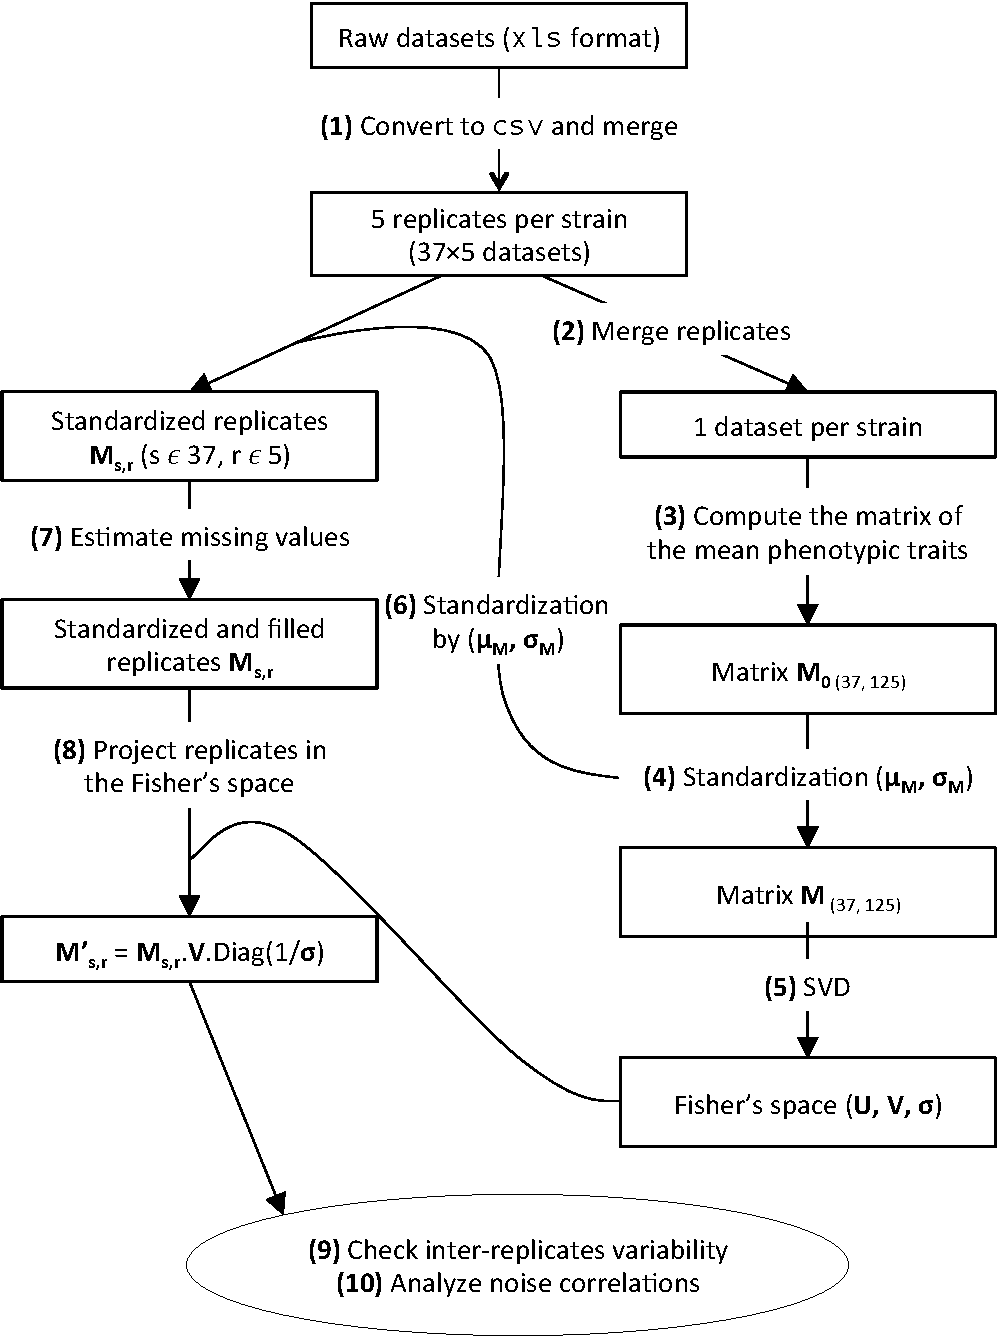
\includegraphics[scale=0.75]{part1_appendixS1_fig1.pdf}
\end{adjustwidth}
\caption[Step-by-step protocol used to analyze single-cell data.]{
\textbf{Step-by-step protocol used to analyze single-cell data.}
\textbf{(1)} Each \texttt{xls} file is converted into \texttt{csv} format, the three files related to each replicate being merged to obtain a single dataset $\boldsymbol{M_{0,s,r}}$ ($s \in \{1,...,m=37\}$, $r \in \{1,...,5\}$) per replicate.
\textbf{(2)} The 5 replicates of each strain are merged to obtain a single dataset per strain.
\textbf{(3)} The matrix $\boldsymbol{M_0}$ of the mean phenotypic trait values per strain is computed.
\textbf{(4,6)} Datasets are standardized according to the mean vector $\boldsymbol{\mu_M} \in \mathbb{R}^{125}$ and the standard deviation vector $\boldsymbol{\sigma_M} \in \mathbb{R}^{125}$ of $\boldsymbol{M_0}$.
\textbf{(5)} A singular values decomposition (SVD) is computed from standardized inter-strain dataset $\boldsymbol{M}$ (see above for the details of the SVD).
\textbf{(7)} Replicate missing values are estimated (see above).
\textbf{(8)} Each replicate dataset is projected into Fisher's space.
\textbf{(9)} Inter-replicate variability is evaluated to ensure that experimental variability is low enough.
\textbf{(10)} Intra-strain phenotypic noise correlations are analyzed.
}
\label{part1:appendixS1:fig1}
\end{figurehere}

%%%%%%%%%%%%%%%%%%%%%%%%%%%%

\newpage

\begin{figurehere}
\begin{adjustwidth}{-0in}{0in}
\centering
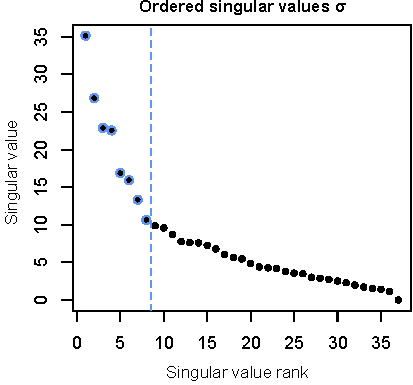
\includegraphics[scale=1.5]{part1_appendixS1_fig2.pdf}
\end{adjustwidth}
\caption[Ordered singular values contained in $\boldsymbol{\sigma}$.]{
\textbf{Ordered singular values contained in $\boldsymbol{\sigma}$.}
A simple empirical method to keep only significant variations is to isolate all the singular values located before the shoulder point in the ordered plot (as shown by a blue dashed line). Here, we kept the first 8 singular values.
}
\label{part1:appendixS1:fig2}
\end{figurehere}

%%%%%%%%%%%%%%%%%%%%%%%%%%%%

\newpage

\begin{figurehere}
\begin{adjustwidth}{-0in}{0in}
\centering
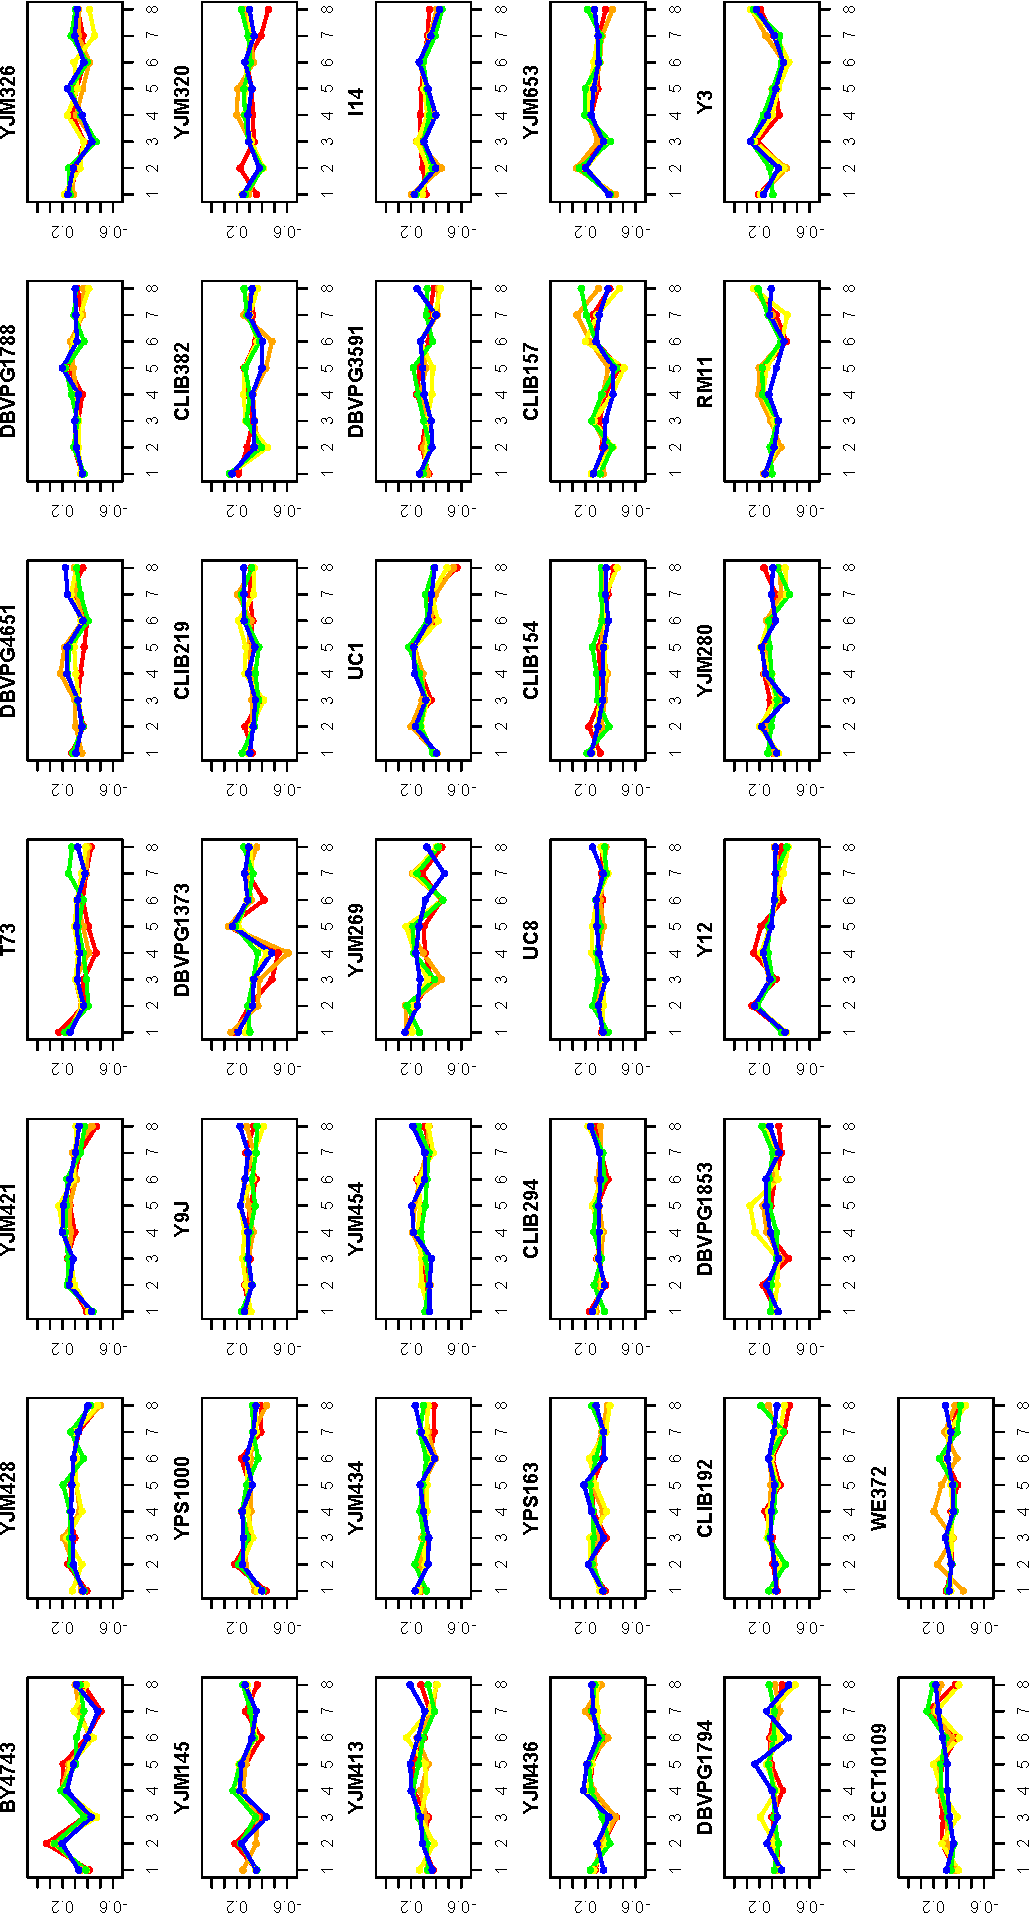
\includegraphics[scale=0.65]{part1_appendixS1_fig3.pdf}
\end{adjustwidth}
\caption[Mean phenotypic trait values per replicate per strain.]{
\textbf{Mean phenotypic trait values per replicate per strain.}
For each replicate of each strain, the mean phenotypic trait values are plotted (one color per replicate on each plot, one plot per strain).
}
\label{part1:appendixS1:fig3}
\end{figurehere}

%%%%%%%%%%%%%%%%%%%%%%%%%%%%

\newpage

\begin{figurehere}
\begin{adjustwidth}{-0in}{0in}
\centering
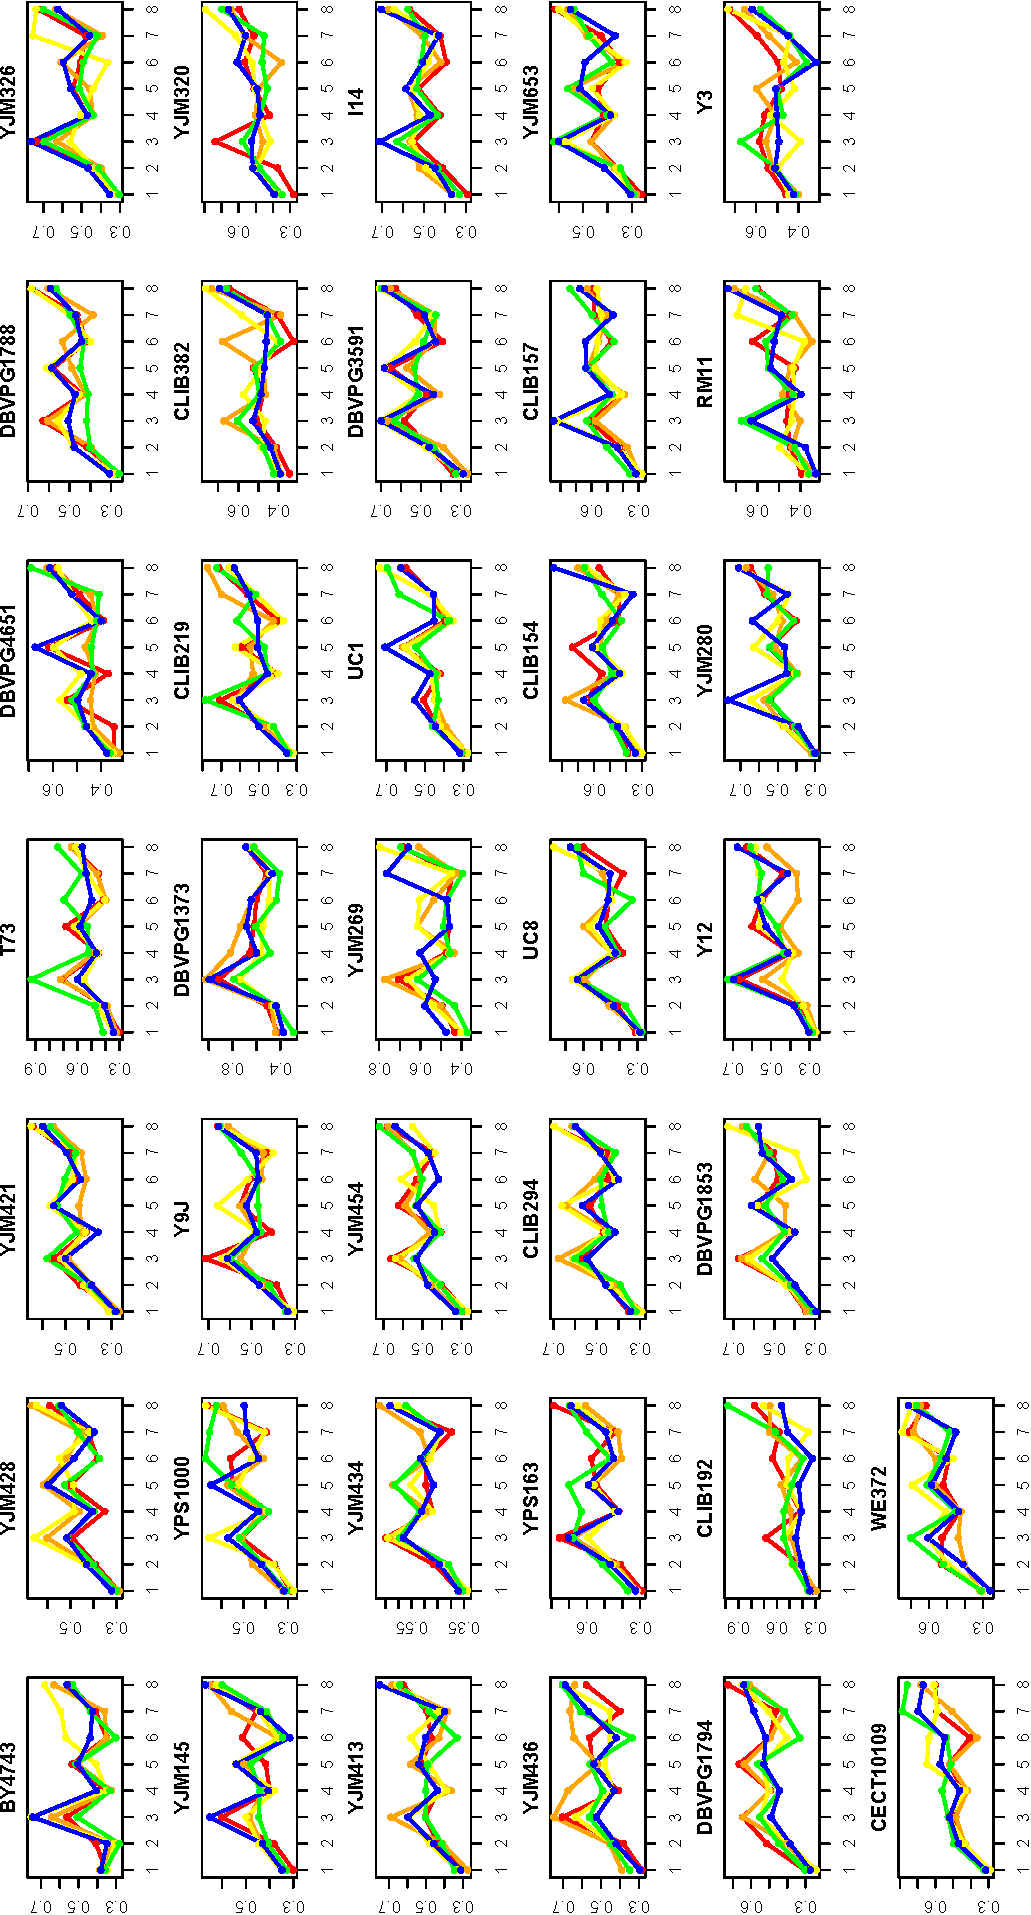
\includegraphics[scale=0.65]{part1_appendixS1_fig4.pdf}
\end{adjustwidth}
\caption[Standard deviation of each phenotypic character per replicate per strain.]{
\textbf{Standard deviation of each phenotypic character per replicate per strain.}
For each replicate of each strain, the standard deviation of each phenotypic character is plotted (one color per replicate on each plot, one plot per strain).
}
\label{part1:appendixS1:fig4}
\end{figurehere}

%%%%%%%%%%%%%%%%%%%%%%%%%%%%

\newpage

\begin{figurehere}
\begin{adjustwidth}{-0in}{0in}
\centering
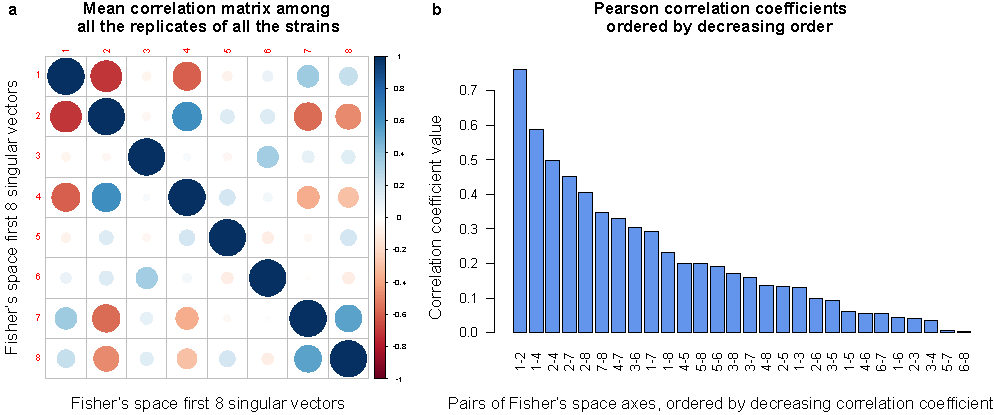
\includegraphics[scale=0.9]{part1_appendixS1_fig5.pdf}
\end{adjustwidth}
\caption[Mean phenotypic noise correlations in the Fisher's space.]{
\textbf{Mean phenotypic noise correlations in the Fisher's space.}
\textbf{a,} The mean correlation matrix across all the replicates of all the strains has been computed and plotted here. For each pair of characters, the strength of the correlation is symbolized by the size of the corresponding circle. A blue color indicates a positive correlation, and a red color a negative correlation.
\textbf{b,} All off-diagonal pairwise correlations between the first 8 axes of Fisher's space are sorted by decreasing order. The most correlated axes in mean are axes 1 and 2 (called PC1 and PC2).
}
\label{part1:appendixS1:fig5}
\end{figurehere}

%%%%%%%%%%%%%%%%%%%%%%%%%%%%

\newpage

\begin{figurehere}
\begin{adjustwidth}{-0in}{0in}
\centering
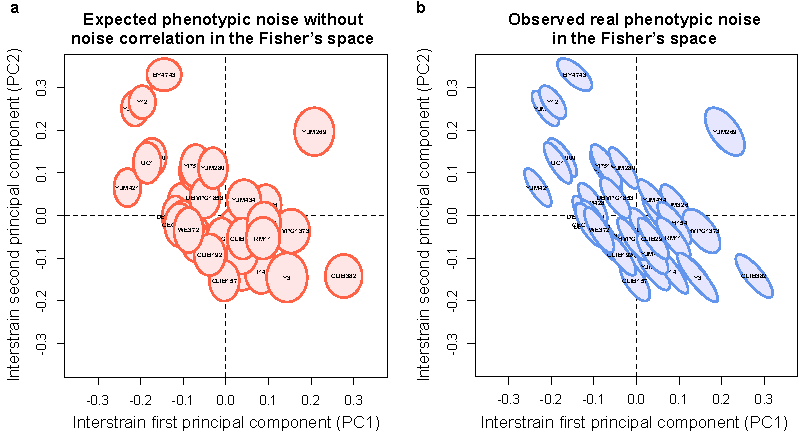
\includegraphics[scale=1]{part1_appendixS1_fig6.pdf}
\end{adjustwidth}
\caption[Yeast intra-strain phenotypic noise is correlated in the Fisher's space.]{
\textbf{Yeast intra-strain phenotypic noise is correlated in the Fisher's space.}
A singular value decomposition (SVD) was performed on the mean trait values of each of the 37 yeast strains. This space is similar to the phenotypic space used in Fisher's geometric model, where phenotypic characters mutate independently and with the same amplitude (\textit{i.e.} mean phenotype mutations are isotropic in this space). For this reason, we called this space ``Fisher's space''. We then projected single-cell data of each strain in this space. We identified the two axes showing the highest noise correlation in mean, for all strains: they correspond to the two first components of Fisher's space (PC1 and PC2).
\textbf{a,} Expected phenotypic noise for each strain without noise correlation between Fisher's space axes (each axis representing a linear combination of phenotypic characters). The shape of the phenotypic noise of each strain is symbolized by an ellipse representing the standard deviation of the associated bivariate normal law. Each ellipse is tagged with the corresponding strain name. The size of the ellipses are rescaled by a factor 0.002 to better distinguish them. The coordinates of the center of each ellipse correspond to the real position of the corresponding strain in Fisher's space (from real data).
\textbf{b,} Real observed phenotypic noise is represented, showing noise correlation between PC1 and PC2 axes, for all the strains.
}
\label{part1:appendixS1:fig6}
\end{figurehere}

